\documentclass[twoside]{article}

\usepackage[sc]{mathpazo} 
\usepackage[T1]{fontenc} 
\linespread{1.10} 
\usepackage{microtype} 

\usepackage[hmarginratio=1:1,top=32mm,columnsep=20pt]{geometry} 
\usepackage{multicol}
\usepackage{graphicx}
\usepackage[hang, small,labelfont=bf,up,textfont=it,up]{caption} 
\usepackage{booktabs} 
\usepackage{float} 
\usepackage{hyperref} 

\usepackage{lettrine} 
\usepackage{paralist} 

\newenvironment{Figure}
  {\par\medskip\noindent\minipage{\linewidth}}
  {\endminipage\par\medskip}

\usepackage{abstract} 
\renewcommand{\abstractnamefont}{\normalfont\bfseries} 
\renewcommand{\abstracttextfont}{\normalfont\small\itshape} 

\usepackage{titlesec} 
\renewcommand\thesection{\Roman{section}} 
\renewcommand\thesubsection{\Alph{subsection}} 
\titleformat{\section}[block]{\large\scshape\centering}{\thesection.}{1em}{} 
\titleformat{\subsection}[block]{\large}{\thesubsection.}{1em}{} 

\usepackage{fancyhdr} 
\pagestyle{fancy} 
\fancyhead{} 
\fancyfoot{} 
\fancyhead[C]{Semester Project $\bullet$ January 2016} 
\fancyfoot[RO,LE]{\thepage} 

%----------------------------------------------------------------------------------------
%	TITLE SECTION
%----------------------------------------------------------------------------------------

\title{\vspace{-15mm}\fontsize{18pt}{10pt}\selectfont\textbf{Developing a Web Platform to Detect Plagiarism on Massive Open Online Course for Java Programs}} 

\author{
\large
\textsc{Alexis Poncet\vspace{2mm}} \\
\normalsize Computer-Human Interaction in Learning and Instruction Laboratory \\ 
\normalsize \href{mailto:alexis.poncet@epfl.ch}{alexis.poncet@epfl.ch} 
\vspace{-5mm}
}
\date{}

%----------------------------------------------------------------------------------------

\begin{document}

\maketitle % Insert title

\thispagestyle{fancy} % All pages have headers and footers

%----------------------------------------------------------------------------------------
%	ABSTRACT
%----------------------------------------------------------------------------------------

\vspace{0.9cm}
\begin{abstract}

MOOCs (massive open online course) is a way to share high-level learning widely and support traditional classrooms where professors are searching solutions to grade equitably each student. However, today, no solution exists to detect automatically plagiarism of source code. In this paper, we study a plagiarism detection tool named \textit{JPlag}, we increase its performance from two minutes to five seconds for 1'300 students submissions and we build a web interface using Django. Given the tight scheduled of professors, we think there is a great value in terms of time saving and the software can be easily adapted in MOOCs.
\vspace{0.5cm}
\end{abstract}

%----------------------------------------------------------------------------------------
%	ARTICLE CONTENTS
%----------------------------------------------------------------------------------------

\begin{multicols*}{2} % Two-column layout throughout the main article text

\section{Introduction}
Today's quick access to information via the internet has made it progressively more tempting for undergrads to commit plagiarism. Controlling falsification became puzzling due to the growing number of students and assignments submitted each day through web platforms; motivating the creation of the application described here.

This paper explains the structure of a new application for detecting plagiarism of students' automated assessment made on Java Programs. The most adapted tool in this contexte is, JPlag, used to compare similarities between several Java Programs. Our work consisted mainly to reevaluate JPlag's, to improve it's comparing performance and to reduce potential time delays when used for large database scheme.

We began by evaluating JPlag original performance on our dataset. We continued by conceptualising and creating the local database. Simultaneously we coded for the web platform using python 1.8.5 and web languages ; html 5, css 3, JavaScript and jQuery.  

Initially JPlag allows to submit and compare about 1'300 assignments within three minutes. However the time necessary to compare a new submission to a 1'000 stored in the database differs greatly from the time needed in an inverse situation. In that case JPlag runs twice its detection plagiarism algorithm on more than 1'000 submissions in the first case scenario, it is twice less efficient than in the inverse scenario. 

JPlag parses each students' work and contrasts it with the data already instaured in the program and does the same process for the already saved information after each new submission. The repeated analyses is unnecessary, what leads to a significant time lost. Consequently, it became clear that the program was lacking memory space where the information from former entries would be stored. In conclusion, forcing the program only to compare new entries with the database would allow to avoid a significant time loss.

\newpage
\section{Problem}

JPlag is an open-source system that finds similarities among multiple sets of source code files. It takes into account programming language syntax and program structure and hence is robust against many kinds of attempts to disguise similarities between plagiarized files. It contains different modules. In fact, we can analyze cpp files, csharp files, java 1.2, java 1.5, java 1.7 files, scheme files, natural language text files and even more if we add the grammar to the application. 

In our researches and in this paper, we just used the java 1.7 version. On the one hand, submitted files by students are java programs, and on the other hand java v1.7 is the latest available version of java implemented in the JPlag tool. To run the application, JPlag requires a minimal configuration, i.e. it needs Java Standard Edition Runtime Environment 7 or older.   

JPlag is a very useful tool when we have to take and compare n programs together in order to detect some similarities. In fact, this system works very well in the case of our current directory contains already each program file. Morever time of tokenizing and comparing are short. So we may ask why not reuse entirely JPlag source code ? 

The answer is that JPlag is not specially designed and created for Massive Open Online Course. In MOOCs, when a student wants to give his work, he sends working files and they are saved on the platform. That means we constantly have students submissions during a deposit period concerning an assignment. Running JPlag at each file sending is not sufficient because we have to execute the software analysis at each time. Notice that JPlag tokenizes and compares all submission files from a folder, even if they already have been tokenizing and comparing to each other previously. Our main issue is this paper is to reduce this waste of time. 

\vspace{0.5cm}
\section{Methods}

\subsection{Performance analysis}

Firstly, we studied original performance of JPlag. We tested the software program with three different sets of assignment representing real EPFL student homework submissions and checked executing time. Notice that each set contains approximately 1'300 submissions including one or more java files. 

In order to test the performance, first we convert all linux executable submission files to java source code files (.java) using a bash script. If we want to specify the programming language, we have to use the command option -l version. Thus, JPlag process knows which module to use. As users make java programs, we only worked on java programs and we did not need to specify version because by default, JPlag uses the latest available version of java (1.7). In consequence, the command line is just : java -jar jplag <root-submissions-dir>. 

We got JPlag source code from github and compiled it with maven. Next, we launched the jplag analysis on a computer with a processor 2.8 GHz Intel Core i7 (Turbo Boost up to 3.3 GHz) and a random access memory of 8GB 1600 MHz DDR3. We timed the process and splitted full time into two categories ; the first one is time of JPlag to tokenize (i.e splits the program to a sequence of tokens) every input files in a matrix and the second one is time making of the software program to compare every column on this matrix. 

\subsection{Preliminary approach to improvement}

We discussed about the right performing process to decrease running time. During the executing time of JPlag, we could see many disk IO. It takes a lot of time. This is caused by some errors during the tokenizing part. In our experimentations, we do not care about error messages. We just want to get the rate of similarities between student's input files. However, the error messages displayed process is generated by antlr, a maven plugin. 

JPlag process was not as longer as we taught before the experiment. In fact, JPlag takes approximately two minutes to find similarities between more than 5'000 files and a little more time if the set of data contains tokenizing errors. However, \textbf{the main problem is that processing time was exactly the same when we submit the first 1'000 files and when we already have 1'000 files in the database and we submit one more.} That is a big issue because the goal of the teacher is exactly to add one more submission at each time. 

The conclusion of this analysis is that JPlag is a very good tool, but insufficient in MOOC context. Therefore, we decided to create our own web platform and reuse the core of JPlag analysis with the aim of detecting plagiarism behaviour in MOOCs and at the same time increasing tokenizing and comparison performance.  

The web platform has been developed with Django 1.8.5, a web python framework on the server side, and with HTML 5, CSS 3, JavaScript, JQuery, Ajax on the client side. Django is scalable, reliable, easy-to-use tool. The real advantage of this framework is the possibility of using bash commands when we want make some operations on our directories. 

Before developing the web platform, we conceptualized the local database of Django. The aim of the database is to save all similarities between submissions concerning one assignment. 

Therefore, we want to retain former similarities. Our model is on the following figure. 
\begin{Figure}
 	\centering
 	\fbox{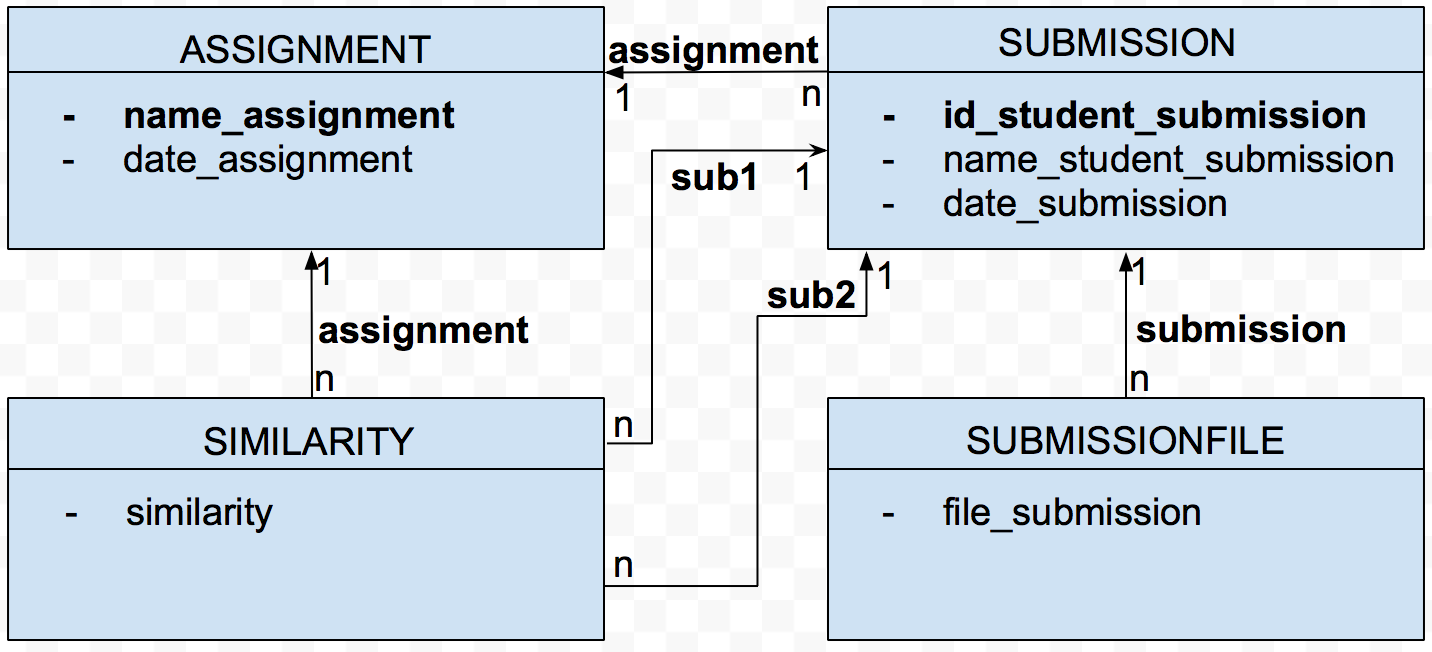
\includegraphics[width=7cm]{./database.png}}
 	\captionof{figure}{Database model}
\end{Figure}
Each bold field on Figure 1 keeps and maintains the integrality of data. Indeed, for instance one submission concerns just one assignment and one student (id). Theses fields are not the real primary keys but have exactly the same function. They are unique. 

Once the database is created, we conceive the web interface structure as we present a mockup in Figure 2.
\begin{Figure}
 	\centering
 	\fbox{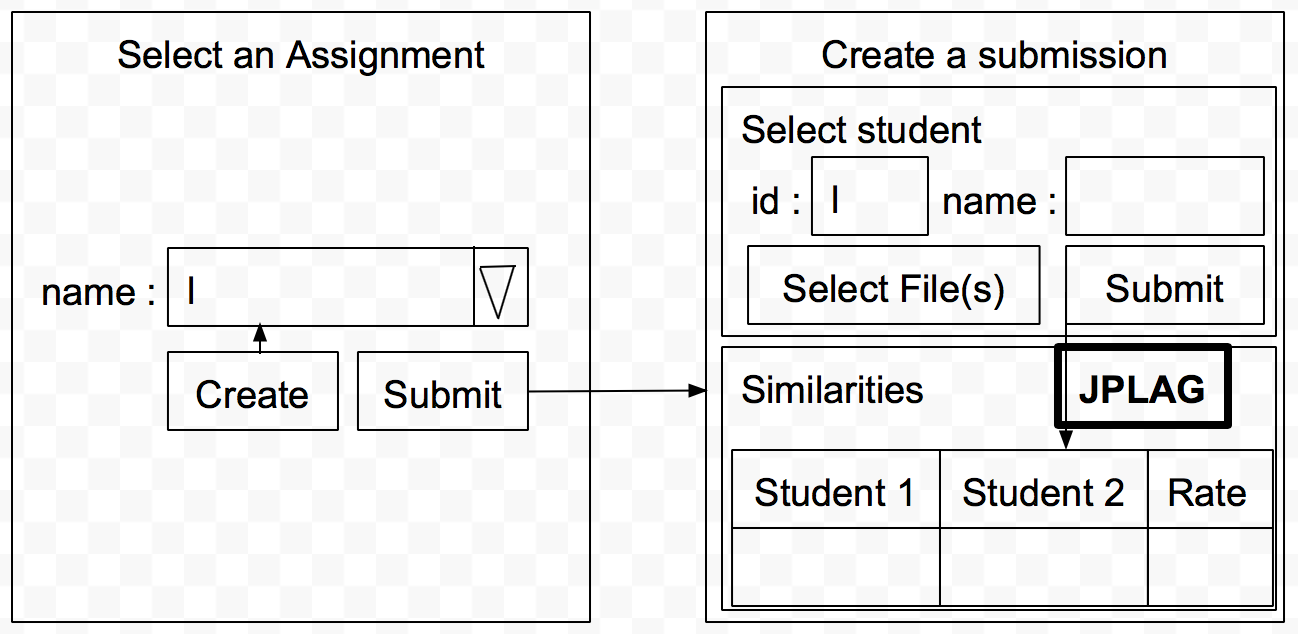
\includegraphics[width=7cm,height=4cm]{./interface.png}}
 	\captionof{figure}{Interface model}
\end{Figure}

\subsection{JPlag problem's}

Original JPlag source code takes every submissions of one assignment and runs analysis for detecting similarities between submissions. The real problem is the lack of memory when we run JPlag because the software tokenizes and compares n submissions at each execution. In other words, finding similarities among n sets of source code files can be splited in two steps. First is the previous JPlag execution (with n-1 submissions). Second is tokenize and compare previous submissions with the new one. With a linear complexity for tokenizing part and a quadratic complexity for comparing part, that means time of JPlag grows polynomially when we increase the number of submissions. 

In our researches, we just want to have similarities between former submissions and the new one.

\newpage
\subsection{One solution : serialization}

JPlag is written in Java language. One famous process to save former results and have a non volatile memory of data is the serialization. To achieve this, we create automatically a folder named $ serializable $ for each assignment, which contains all former data. 

Moreover, we pose some requirements. Firstly, all data and each attribute inside want to be serializable and in consequence have to implement the serializable interface. That is why Submission, Parser, Structure and Language (java 1.7) classe's are becoming serializable classes. 

Secondly, some java parameters are mandatory. We have to know each previous submission and the number of former submissions. Concerning the first point, it is very simple because we store directly the matrix of submissions after the tokenizing part in a file named $ Design\_data.ser $. The second point is easy too because we just have to know the length of the matrix. We save this parameter in another file named $ Design\_errorsNumber.ser $, which contains also the number of general errors, such as tokenizing errors and comparison errors for statistics. 

At each execution of JPlag, whether files exist, we get data from these files and we initialize the matrix of submissions and index comparison. If files do not exist, we run original JPlag analysis and we create serializable files. Finally, JPlag results are stored in our database and are shown to the user on the web platform. 
\vfill

\subsection{One more problem : deleting submissions}

Serialization solves the main problem but what would happend when we removed one student submission already analysed by JPlag from the selected assignment ? The vector of submissions will become wrong because it will have incorrect data in the current context of the analysis. 

To tackle this problem, we edited JPlag source code. When we get serializable data, we verify that each former submission's directory is still located in the assignment folder. If we do not find the submission folder, it means that a person removed student directory corresponding to the submission. At the next JPlag execution, we will delete data concerning it inside the matrix of submissions. By this way, we are sure to always have right data stored, even if a person makes some modifications before or after running JPlag tool.

\subsection{Another JPlag platform : the administration part}

The django administration interface allows us to manage entirely the database and to execute JPlag analysis at each new modification, the same way as the web interface. The design is based on CRUD (Create Read Update Delete) process. Indeed, when we create or update a submission or a file we run JPlag at back end. Then either new similarities are stored into the database or former similarities are substituted by new output of JPlag tool. Concerning deleting process, refer to the previous section. 

Moreover, we modified rights of similarity table with the read-only property in order to refuse any manual modifications and having only JPlag output data. Thereby, we always have a great integrality of data in our local database.
\vfill

%------------------------------------------------

\newpage
\section{Results}

\subsection{Pre Analysis}

Before implementing the tool, we focused on JPlag's original process and consequently ran this process at the beginning of the project with three large sets of data. For future reference, we timed the process. The full time of JPlag analysis depends on the number of submitted files and disk IO errors. Figure 3 compares experimentations of original JPlag's performance.  \\

\begin{table}[H]
\caption{Original JPlag's performance}
\resizebox{7cm}{!}{
\begin{tabular}{lccccc}
\toprule
 & \multicolumn{2}{c}{Number} & \multicolumn{3}{c}{Time} \\
\cmidrule(lr){2-3}
\cmidrule(lr){4-6} 
 \begin{tabular}{@{}c@{}} Sets of \\Data \end{tabular} & Students & Files & Tokenizing & Comparing & Total \\
\midrule
 \begin{tabular}{@{}c@{}} \big[00000057\big] \\ Assignment \\ \big[11 31\big] \end{tabular}& 1333 & 5537 & 2m 10s &  12s &  2m 22s \\
 \begin{tabular}{@{}c@{}} \big[00000058\big] \\  Assignment \\ \big[11 32\big] \end{tabular}& 1299 & 5430 & 2m 12s & 22s  &  2m 34s\\
 \begin{tabular}{@{}c@{}} \big[00000059\big]  \\ Assignment \\  \big[11 33\big] \end{tabular}& 1245 & 5717 & 3m 00s & 1m 20s & 4m 20s \\
\bottomrule
\end{tabular}
}
\end{table}

We can see that JPlag analysis takes between two and five minutes to find similarities between more than 5'000 files. When we submit a new student submission with original JPlag, it repeats exactly the same process and get always the same or more number of old errors. Therefore when we submit new files, the JPlag analysis takes more time than previous running, so in this example more than four minutes for one more submission. The serialization method is very helpful in this case because we do not need to launch again former submissions which are contain some errors. 

\subsection{After serialization}

After serialization process implemented, we compare JPlag tool without serialization versus JPlag analysis with serialization. We did experimentation on the first set of data (more quickly than others).

\begin{Figure}
 	\centering
 	\fbox{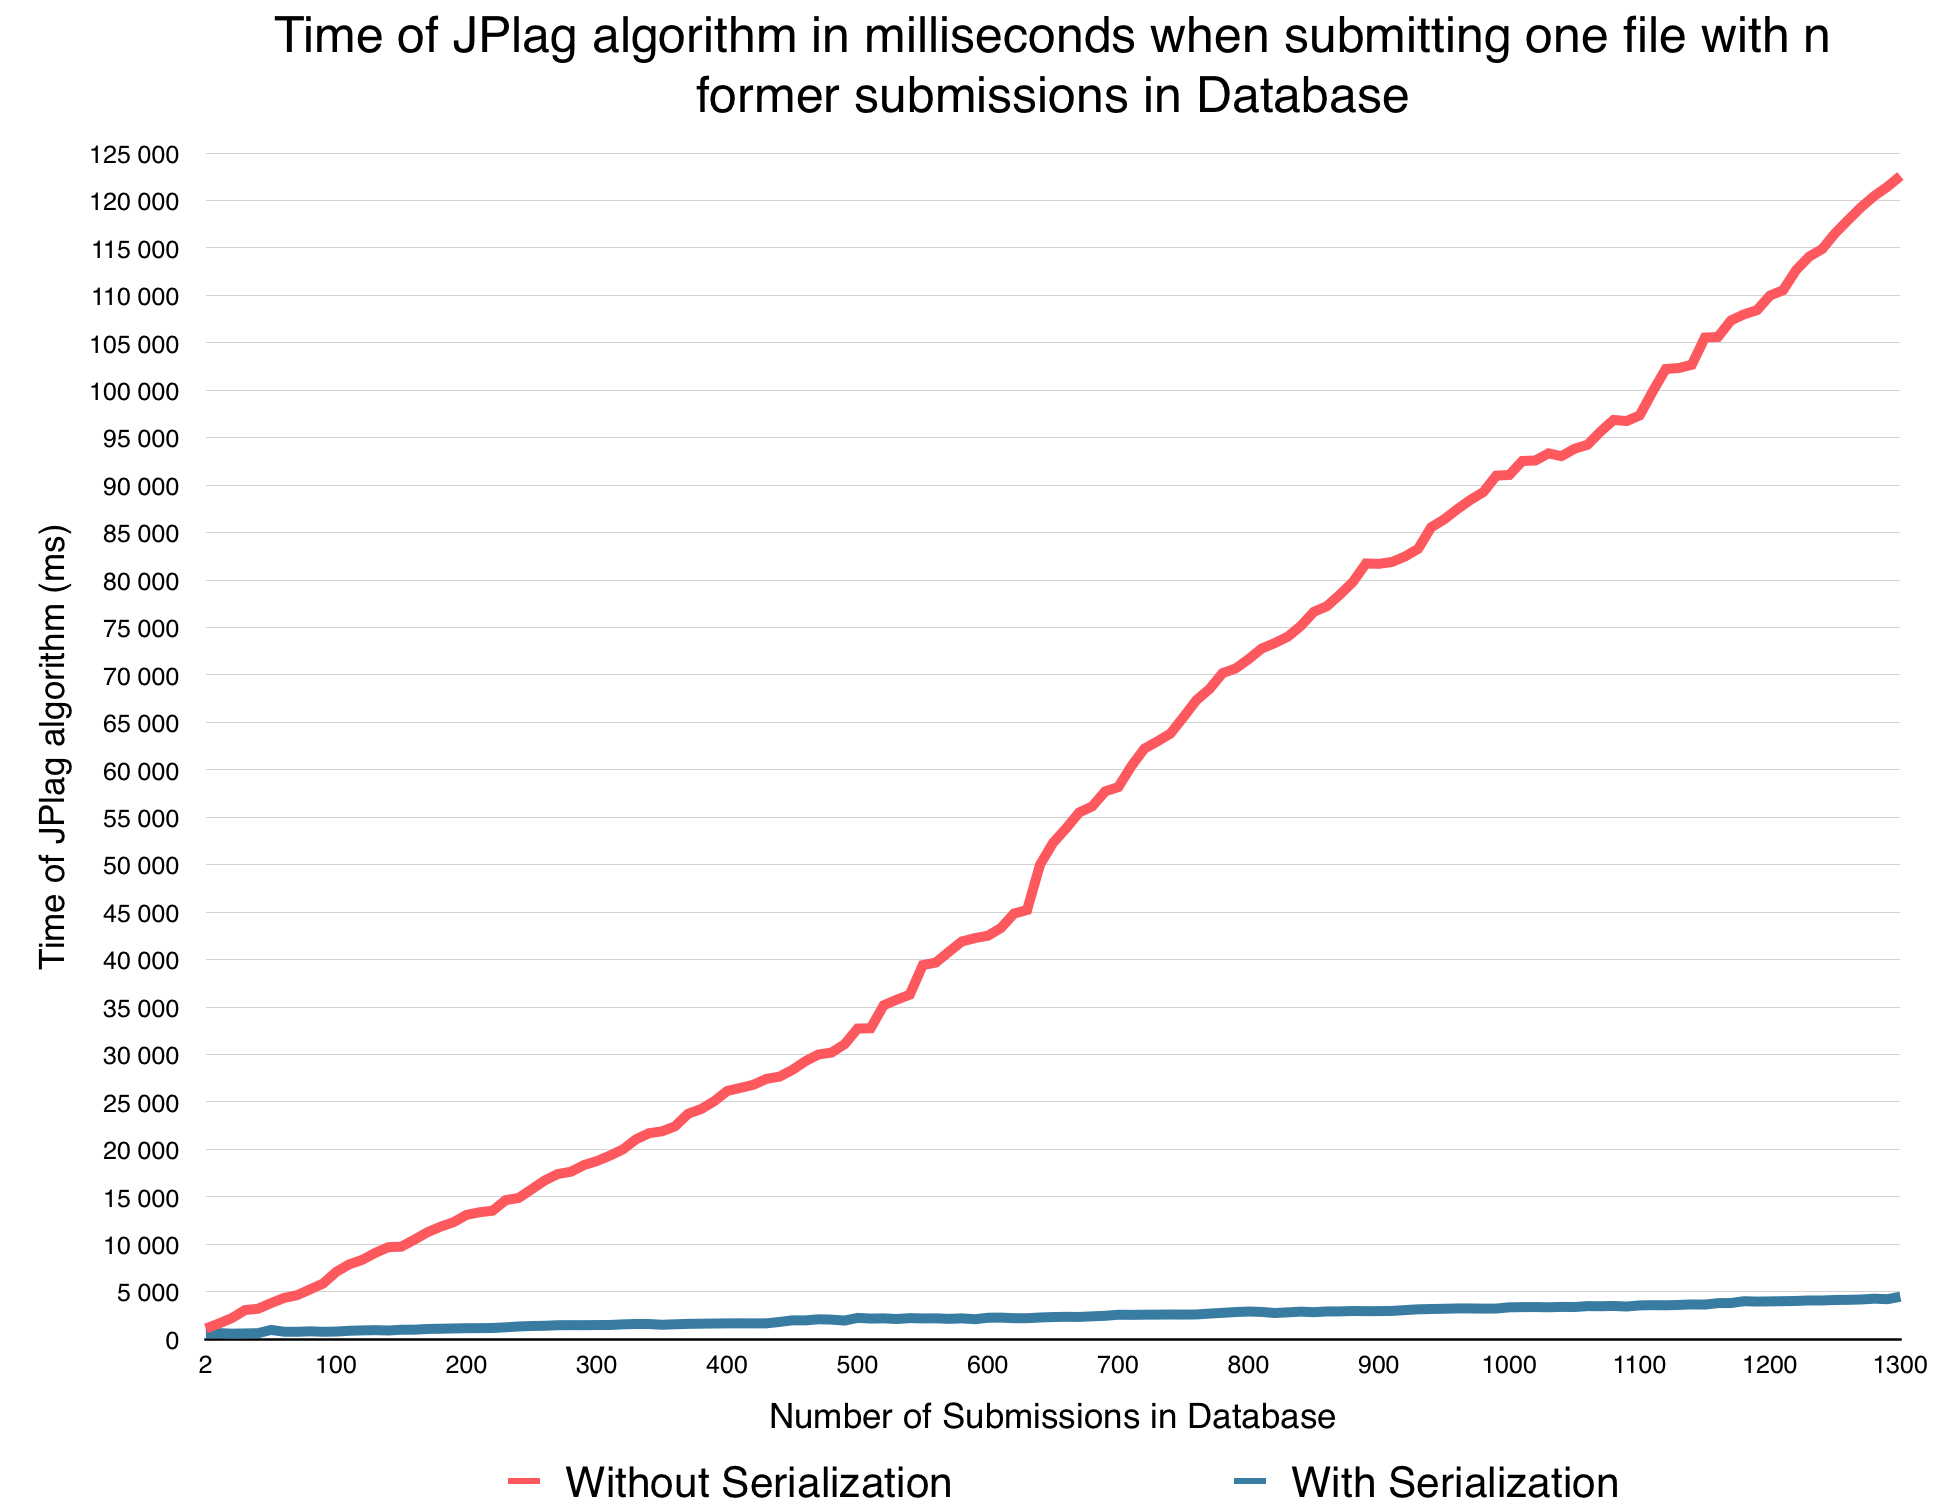
\includegraphics[width=7cm]{./comparisonJplagTime.png}}
 	\captionof{figure}{Comparison of JPlag performance between without serialization process and with serialization process when we submit one more file to the database}
\end{Figure}

In Figure 3, we see that the time of original JPlag analysis grows quadratically according to the number of submissions. On the contrary, time of new JPlag process is linear. In fact, JPlag analysis makes less than five seconds with a big database (1'300 submissions) whereas original JPlag makes more than two minutes. 

Theses results are normal. Indeed, on the one hand, original complexity of tokenizing session is $O(n)$. That means time grows up proportionally to the number of submissions. The initial JPlag analyses more and more submissions at each starter whereas the new process has just to tokenize the last one each time ($O(1)$).

Time complexity of original comparing is $O(n^2)$. That means original JPlag makes time growing very quickly according to the number of submissions. In fact, we compare again n-1 submissions together and then compare the new submission to former submissions. On the contrary, the new JPlag compares only the new submission to previous student submissions. And that is why on the previous figure, we can see that time of JPlag with serialization tool grows very slowly with the number of submissions. 

\newpage
We summarize the complexity in the following table.

\begin{table}[H]
\caption{Complexity of JPlag without serialization and with serialization}
\resizebox{7cm}{!}{
\begin{tabular}{lcc}
 \begin{tabular}{@{}c@{}} Steps of the JPlag Process \end{tabular} & Without Serialization & With Serialization \\
\midrule
Tokenize Part & $O(n)$ & $O(1)$ \\
Comparison Part & $O(n^2)$ & $O(n)$\\
Total & $O(n)$ + $O(n^2)$ $ \sim $ $O(n^2)$  & $O(1)$ + $O(n)$ $ \sim $ O(n)\\
\bottomrule
\end{tabular}
}
\end{table}

To conclude, we reduced time of JPlag from $O(n^2)$ to $O(n)$. The linear complexity is the minimal possible complexity with the aim of finding similarities among multiple sets of source code files.

%------------------------------------------------
\vspace{0.5cm}
\section{Discussion}

As we can see in Table 1 and in Figure 3, JPlag original performances are not perfect. We have some parameters which can have a real impact on JPlag output and on JPlag's performances. The aim of this section is to discuss about all of these and suggest the answers to the problematic which is what are the best way to reduce JPlag executing time on Massive Open Online Course ?

\subsection{Number of submissions}

The main parameter is the number of submissions. In fact, JPlag processing time mostly depends on the number of student submissions. More we have submissions, the higher is the time of tokenize and comparison part. 

To minimize the weight of this parameter into the process, we implemented the serialization. Indeed, as we can see in Table 2, we reduce the complexity from $O(n^2)$ to $O(n)$. At each new submission, we are mandatory to tokenize it and compare it with each former submission. Therefore, we can not minimize more executing time process. 
\vfill

\subsection{Number of files}

According to the previous parameter, the number of files is a major hidden parameter because JPlag has to make trivial I/O operations, such as open a file, read it and close it, which take some time. More we have files, the higher is the I/O latence time. Obviously this time depends on the device on which we make experimentation and consequently we do not have the control on this parameter. In our researches, we make every experiment on a basic laptop with a processor 2.8 GHz Intel Core i7 and 8go of random access memory. \\

However, the number of submissions and files are not unique parameters and it exists other less obvious parameters. Indeed, it is very difficult to reduce the time of the comparison process because it needs few technical specificities. Besides, comparison part is not the longest part of the JPlag analysis unlike the tokenize part. That is why the two next parameters are focused on the tokenize part.

\subsection{Tokenize part : Length of files}

Additionally to the number of files, the length of submission files is very important. Indeed, JPlag process looks over each file and at the same time splits the program to a sequence of tokens. More source code input file contains characters, the higher is the time of tokenizing.

In our researches, we can not check the length of each file but we consider they contain approximatively the same number of characters. In fact, our data corresponding to student's little homeworks, which are java programs and consequently can not contain so much characters.
\vfill

\newpage
\subsection{Tokenize part : I/O operations}

In our examples, the last set of data contains more token recognition errors than the first two. And that is why time of JPlag's execution is larger. One output error is not significant. However, if you repeat it n times, it becomes really important and takes a lot of time. Indeed, computer buses are originally slow and are used to communicate from open files to the buffer. Therefore, with so many interactions, buses are busy and make some I/O bottlenecks, that result in a waste of time. We have to think about all cases as much as possible. Unfortunately we have no control over error recognition. And that we could see on the last scenario. Errors are in student files. 

Therefore, we can place ourselves in the most of pessimistic case and think that each student submission file can contains so many errors. In this case, we are sure that the first two and the last case scenario's time are higher than in our experiment. However the complexity is $O(n)$, it means that time grows up very quickly when we make some I/O operations on disk. 

After our researches and our serialization, time generated by errors is mostly lower than original JPlag process and stay insignificant.

\subsection{Multi-threading}

During our researches, we also considered another method of JPlag execution. We know that submissions are independent to each other. That means that in theory on one hand we can tokenize every submission file separately and on the other hand get each output previous process and compare them. 

Before implementing this process thanks to multi threading method in java, we made the experimentation with a little bash scripting. Unfortunately, this test was not efficient. Core of the device experiments was not sufficient and the JPlag process took more time than expected. 

However we think that this solution can be better than serialization process in some case. For instance, when we run JPlag on a new submission, serialization is more efficient than multi threading because we just have one thread, whereas multi-threading can be more efficiently than serialization concerning JPlag's execution on several new submissions.


%------------------------------------------------
\vspace{0.5cm}
\section{Conclusion}

In conclusion, original JPlag works successfully for finding similarities among multiple sets of source code files already present in a folder. However, MOOCs allow students to submit files when they want and consequently need frequent update of similarities behaviour analysis. That is why we decided to use the core of JPlag open-source tool and we adapted the program to the MOOCs. We searched which parameters have a real impact on the execution time and then made some experimentation with the aim to reduce JPlag processing time. 

Final solution is the serialization. Indeed, we serialize the tokenize part of JPlag and do not run again former similarities analysis. Thus, we have very good process with no waste of time and really adapted to Massive Open Online Course. We reduced JPlag executing time from two minutes to five seconds when submiting one more submission into a large database with approximatively 1'300 submissions - 5'000 files. This reduction is due to the complexity sag, switched from quadratic complexity to linear complexity - the optimal solution for this kind of process.


%----------------------------------------------------------------------------------------
%	REFERENCE LIST
%----------------------------------------------------------------------------------------

\vspace{0.5cm}
\begin{thebibliography}{99} % Bibliography - this is intentionally simple in this template

\bibitem[1]{}
S. Jain, M. Singhal and A. Shah,
\newblock {\itshape"Exploring the Usage of Existing Plagiarism Tools for
Automated Student Assessment for Java Program"}, International Journal of Information and Education Technology, Vol. 6, No. 3, March 2016.
 
\end{thebibliography}

%----------------------------------------------------------------------------------------

\end{multicols*}

\end{document}

